\chapter{KẾT QUẢ VÀ BÀN LUẬN}
\label{ch:ket_qua}

\section{Kết quả tổng quan}

Bảng~\ref{tab:tongquan} tập hợp kết quả của cả năm cấu hình, đo bằng pycocotools trên cùng một tập
kiểm tra gồm 638 ảnh, trong cùng một lượt chạy.

\begin{table}[H]
\centering
\caption{Kết quả năm cấu hình đo bằng pycocotools trên tập kiểm tra}
\label{tab:tongquan}
\footnotesize
\begin{tabular}{lrrrrrrr}
\toprule
\textbf{Cấu hình} & \textbf{Tham số (M)} & \textbf{Tệp (MB)} & \textbf{mAP@0,5} & \textbf{mAP@.5:.95} & \textbf{$AP$ nhỏ} & \textbf{$AP$ lớn} & \textbf{FPS} \\
\midrule
YOLO26s (thầy)        & 9,47 & 19,39 & 0,9520 & 0,7822 & 0,616 & 0,859 & 74,4 \\
YOLO26n đối chứng     & 2,38 & 5,15  & \textbf{0,9348} & \textbf{0,7773} & \textbf{0,548} & \textbf{0,862} & 69,7 \\
YOLO26n chưng cất     & 2,38 & 5,15  & 0,9014 & 0,7450 & 0,486 & 0,852 & 74,8 \\
\midrule
ONNX FP32 (từ trò KD) & ---  & 9,35  & 0,9079 & 0,7473 & 0,462 & 0,847 & 19,8 \\
ONNX INT8 (từ trò KD) & ---  & 2,78  & 0,9041 & 0,7437 & 0,437 & 0,839 & 9,4 \\
\bottomrule
\end{tabular}
\end{table}

\hopnhanmanh{Đọc theo cột mAP@0,5, khoảng cách giữa các cấu hình trông khiêm tốn --- toàn bộ nằm
trong dải 0,90 đến 0,95. Đọc theo cột $AP$ nhỏ, bức tranh khác hẳn: dải trải từ 0,437 đến 0,616,
tức chênh lệch tương đối lớn gấp nhiều lần. Đây là luận điểm trung tâm của báo cáo và sẽ được
định lượng ở Mục~\ref{sec:ap_nho_ket_qua}.}

Cột $AP$ lớn cho thấy điều ngược lại: cả ba mô hình PyTorch đều nằm quanh mức 0,85--0,86, gần như
không phân biệt được, và hai bản ONNX cũng chỉ thấp hơn chút ít. Nói cách khác, với vật thể lớn thì
bài toán đã bão hoà và mọi cấu hình đều giải quyết tốt như nhau. Điều này nhất quán với phân tích
thành phần bộ dữ liệu ở Mục~\ref{sec:thanhphan}: hơn một nửa số hộp bao thuộc nhóm lớn, và chính vì
vậy chúng chi phối mAP tổng đồng thời che lấp mọi khác biệt thật sự.

\section{Chưng cất tri thức}

\subsection{Xác minh cơ chế đã được kích hoạt}

Trước khi diễn giải một kết quả âm, cần loại trừ khả năng cơ chế chưng cất không hề chạy --- nếu
không, ta chỉ đang so sánh hai lần huấn luyện thông thường với kích thước lô khác nhau.

Nhật ký huấn luyện của nhánh chưng cất có thêm cột \texttt{train/dis\_loss}, cột này \emph{không}
tồn tại ở nhánh đối chứng. Giá trị của nó giảm từ \textbf{12,1663} ở chu kỳ đầu xuống
\textbf{1,1608} ở chu kỳ cuối. Vậy hàm mất mát chưng cất đã hoạt động và đã hội tụ; kết quả âm dưới
đây là kết quả thật chứ không phải lỗi cấu hình.

\subsection{Kết quả trái với kỳ vọng}
\label{sec:trai_ky_vong}

Giả thuyết ban đầu là mô hình học trò sẽ hưởng lợi từ phân phối đầu ra mềm của mô hình
thầy~\cite{hinton2015distillation}. Kết quả ngược lại: mô hình được chưng cất đạt mAP@0,5 bằng
0,9014, thấp hơn mô hình đối chứng (0,9348) \textbf{3,34 điểm phần trăm}, và thấp hơn tới
\textbf{6,20 điểm phần trăm} nếu xét riêng $AP$ trên vật thể nhỏ.

\begin{table}[H]
\centering
\caption{Ba phép so sánh cốt lõi}
\label{tab:delta}
\small
\begin{tabular}{lrrr}
\toprule
\textbf{Phép so sánh} & \textbf{$\Delta$ mAP@0,5} & \textbf{$\Delta$ mAP@.5:.95} & \textbf{$\Delta$ $AP$ nhỏ} \\
\midrule
Trò chưng cất so với trò đối chứng & $-0{,}0334$ & $-0{,}0323$ & $\mathbf{-0{,}0620}$ \\
Trò chưng cất so với thầy          & $-0{,}0507$ & $-0{,}0372$ & $\mathbf{-0{,}1308}$ \\
ONNX INT8 so với ONNX FP32         & $-0{,}0038$ & $-0{,}0036$ & $\mathbf{-0{,}0247}$ \\
\bottomrule
\end{tabular}
\end{table}

Có ba cách giải thích khả dĩ cho kết quả này.

\textbf{Thứ nhất, khoảng cách năng lực giữa thầy và trò quá hẹp.} Thầy chỉ đạt 0,9520, tức nhỉnh
hơn trò đối chứng 1,72 điểm phần trăm. Lượng ``tri thức tối'' mà một mô hình chỉ tốt hơn chút ít có
thể truyền đạt là rất nhỏ, trong khi chi phí nhiễu do bắt chước một phân phối không hoàn hảo thì
vẫn phải trả đủ. Đây đúng là điều kiện áp dụng đã nêu ở Mục~\ref{sec:kd_lythuyet}.

\textbf{Thứ hai, kích thước lô không đồng nhất.} Nhánh chưng cất chạy với lô 8 so với 24 của nhánh
đối chứng, do phải nạp đồng thời cả hai mô hình vào bộ nhớ card đồ hoạ. Đây là yếu tố gây nhiễu
chưa kiểm soát được và tự nó đã đủ giải thích một phần chênh lệch. Cần nói thẳng rằng vì yếu tố này,
kết luận ``chưng cất có hại'' \emph{không} được rút ra một cách chắc chắn; điều rút ra được là
``trong cấu hình cụ thể này, chưng cất không mang lại lợi ích''.

\textbf{Thứ ba, hệ số chưng cất có thể quá lớn.} Giá trị 6,0 là mặc định của thư viện, chưa được
quét thử. Với một cặp thầy--trò gần nhau như vậy, thành phần bắt chước có thể đã lấn át tín hiệu từ
nhãn cứng.

\subsection{Kiểm tra ngưỡng chấp nhận}

Năm ngưỡng khai báo trước ở Mục~\ref{sec:nguong_chap_nhan} cho kết quả ba đạt, hai không đạt --- và
cả hai ngưỡng không đạt đều thuộc về giả thuyết chưng cất.

\begin{table}[H]
\centering
\caption{Kiểm tra các ngưỡng chấp nhận khai báo trước khi chạy thực nghiệm}
\label{tab:thresh}
\small
\begin{tabular}{lll}
\toprule
\textbf{Ngưỡng} & \textbf{Giá trị đo} & \textbf{Kết quả} \\
\midrule
KD không kém đối chứng quá 0,005 điểm     & $\Delta = -0{,}0323$ & \textbf{KHÔNG ĐẠT} \\
KD tốt hơn đối chứng (kỳ vọng ban đầu)    & $\Delta = -0{,}0323$ & \textbf{KHÔNG ĐẠT} \\
INT8 giảm không quá 0,015 điểm so với FP32 & giảm $0{,}0036$     & ĐẠT \\
INT8 nhỏ hơn FP32 ít nhất 50\%            & giảm 70,3\%          & ĐẠT \\
Trò chưng cất nhẹ hơn thầy                & 5,15 so với 19,39 MB & ĐẠT \\
\bottomrule
\end{tabular}
\end{table}

Việc khai báo tiêu chí trước và báo cáo cả kết quả không đạt là cách làm đúng đắn về mặt phương
pháp: nó ngăn việc diễn giải lại kỳ vọng sau khi đã nhìn thấy số liệu. Kết quả âm này được giữ lại
thay vì loại bỏ, vì nó xác định rõ \emph{điều kiện áp dụng} của kỹ thuật.

\section{Lượng tử hoá}

\subsection{Đánh đổi giữa dung lượng, tốc độ và độ chính xác}

\begin{table}[H]
\centering
\caption{Ảnh hưởng của việc xuất mô hình và lượng tử hoá}
\label{tab:quant}
\small
\begin{tabular}{lrrrr}
\toprule
\textbf{Cấu hình} & \textbf{Tệp (MB)} & \textbf{mAP@0,5} & \textbf{Trung vị (ms)} & \textbf{p95 (ms)} \\
\midrule
PyTorch FP16 (gốc) & 5,15 & 0,9014 & 13,37  & 14,33 \\
ONNX FP32          & 9,35 & 0,9079 & 50,41  & 55,76 \\
ONNX INT8          & 2,78 & 0,9041 & 106,90 & 112,88 \\
\bottomrule
\end{tabular}
\end{table}

Về dung lượng, lượng tử hoá đạt đúng mục tiêu: 2,78~MB so với 9,35~MB, tức giảm \textbf{70,3\%},
vượt xa ngưỡng 50\% đã đặt ra.

Về tốc độ thì kết quả trái ngược hoàn toàn với kỳ vọng thông thường. Về lý thuyết, biểu diễn số
nguyên 8 bit cho phép dùng các nhân tính toán số nguyên nhanh
hơn~\cite{jacob2018quantization}. Trên thực tế, bản INT8 có độ trễ trung vị 106,90~ms, tức
\emph{chậm hơn} bản FP32 hơn hai lần và chậm hơn bản PyTorch gốc tới tám lần. Đúng như đã dự đoán ở
Mục~\ref{sec:quant_lythuyet}, lợi ích tốc độ của lượng tử hoá chỉ hiện thực hoá khi môi trường thực
thi có nhân số nguyên được tối ưu cho phần cứng đích; nếu không, thời gian tiết kiệm được bị tiêu
hết vào các phép chuyển đổi lượng tử hoá và giải lượng tử hoá xen giữa các lớp.

Cũng đáng lưu ý rằng bản ONNX FP32 đã chậm hơn bản PyTorch gốc gần bốn lần trước khi lượng tử hoá
--- đây là chi phí của việc đổi môi trường thực thi, và chính nhờ có mốc trung gian này mà ta tách
được hai nguyên nhân ra khỏi nhau.

\subsection{Chi phí thật nằm ở vật thể nhỏ}
\label{sec:ap_nho_ket_qua}

Đây là kết quả quan trọng nhất của đề tài.

Nếu chỉ đọc mAP tổng, lượng tử hoá INT8 trông gần như miễn phí: mAP@0,5 giảm 0,0038, tức chưa tới
nửa điểm phần trăm, đổi lại dung lượng giảm hơn 70\%. Bất kỳ ai ra quyết định triển khai dựa trên
con số đó sẽ kết luận rằng INT8 là lựa chọn hiển nhiên.

Nhưng khi tách theo nhóm kích thước, $AP$ trên vật thể nhỏ giảm 0,0247 --- \textbf{gấp 6,5 lần} mức
suy giảm của mAP tổng.

\begin{table}[H]
\centering
\caption{So sánh mức suy giảm giữa mAP tổng và $AP$ trên vật thể nhỏ}
\label{tab:pha_loang}
\small
\begin{tabular}{lrrr}
\toprule
\textbf{Phép can thiệp} & \textbf{$\Delta$ mAP@0,5} & \textbf{$\Delta$ $AP$ nhỏ} & \textbf{Tỉ số} \\
\midrule
Chưng cất tri thức & $-0{,}0334$ & $-0{,}0620$ & 1,9 lần \\
Lượng tử hoá INT8  & $-0{,}0038$ & $-0{,}0247$ & \textbf{6,5 lần} \\
\bottomrule
\end{tabular}
\end{table}

\hopnhanmanh{Ở cả hai phép can thiệp, mức suy giảm trên vật thể nhỏ đều lớn hơn hẳn mức suy giảm
trên mAP tổng. Hệ quả thực tiễn rất cụ thể: với bài toán biển báo giao thông, nơi biển ở xa quyết
định thời gian phản ứng của xe, một quyết định triển khai chỉ dựa trên mAP tổng có nguy cơ sai
nghiêm trọng. Phải đọc $AP$ tách theo nhóm kích thước.}

Cơ chế đằng sau hiện tượng này đã được dự đoán từ lý thuyết ở Mục~\ref{sec:quant_lythuyet}: sai số
lượng tử hoá tác động lên toàn bộ bản đồ đặc trưng, trong khi vật thể nhỏ vốn chỉ để lại tín hiệu
yếu trên bản đồ đó, nên tỉ lệ tín hiệu trên nhiễu của chúng suy giảm nhiều hơn. Việc quan sát thực
nghiệm khớp với dự đoán lý thuyết làm tăng độ tin cậy của kết luận.

Lý do mAP tổng che giấu được điều này cũng đã rõ từ Chương~\ref{ch:phuong_phap}: 51,30\% số hộp bao
trong bộ dữ liệu thuộc nhóm lớn, và $AP$ trên nhóm đó gần như không đổi (0,847 so với 0,839). Nhóm
dễ chiếm đa số nên nó chi phối giá trị trung bình và pha loãng suy giảm ở nhóm khó.

\section{Phân tích lỗi}

\subsection{Nhầm lẫn giữa các lớp}

\begin{figure}[H]
\centering
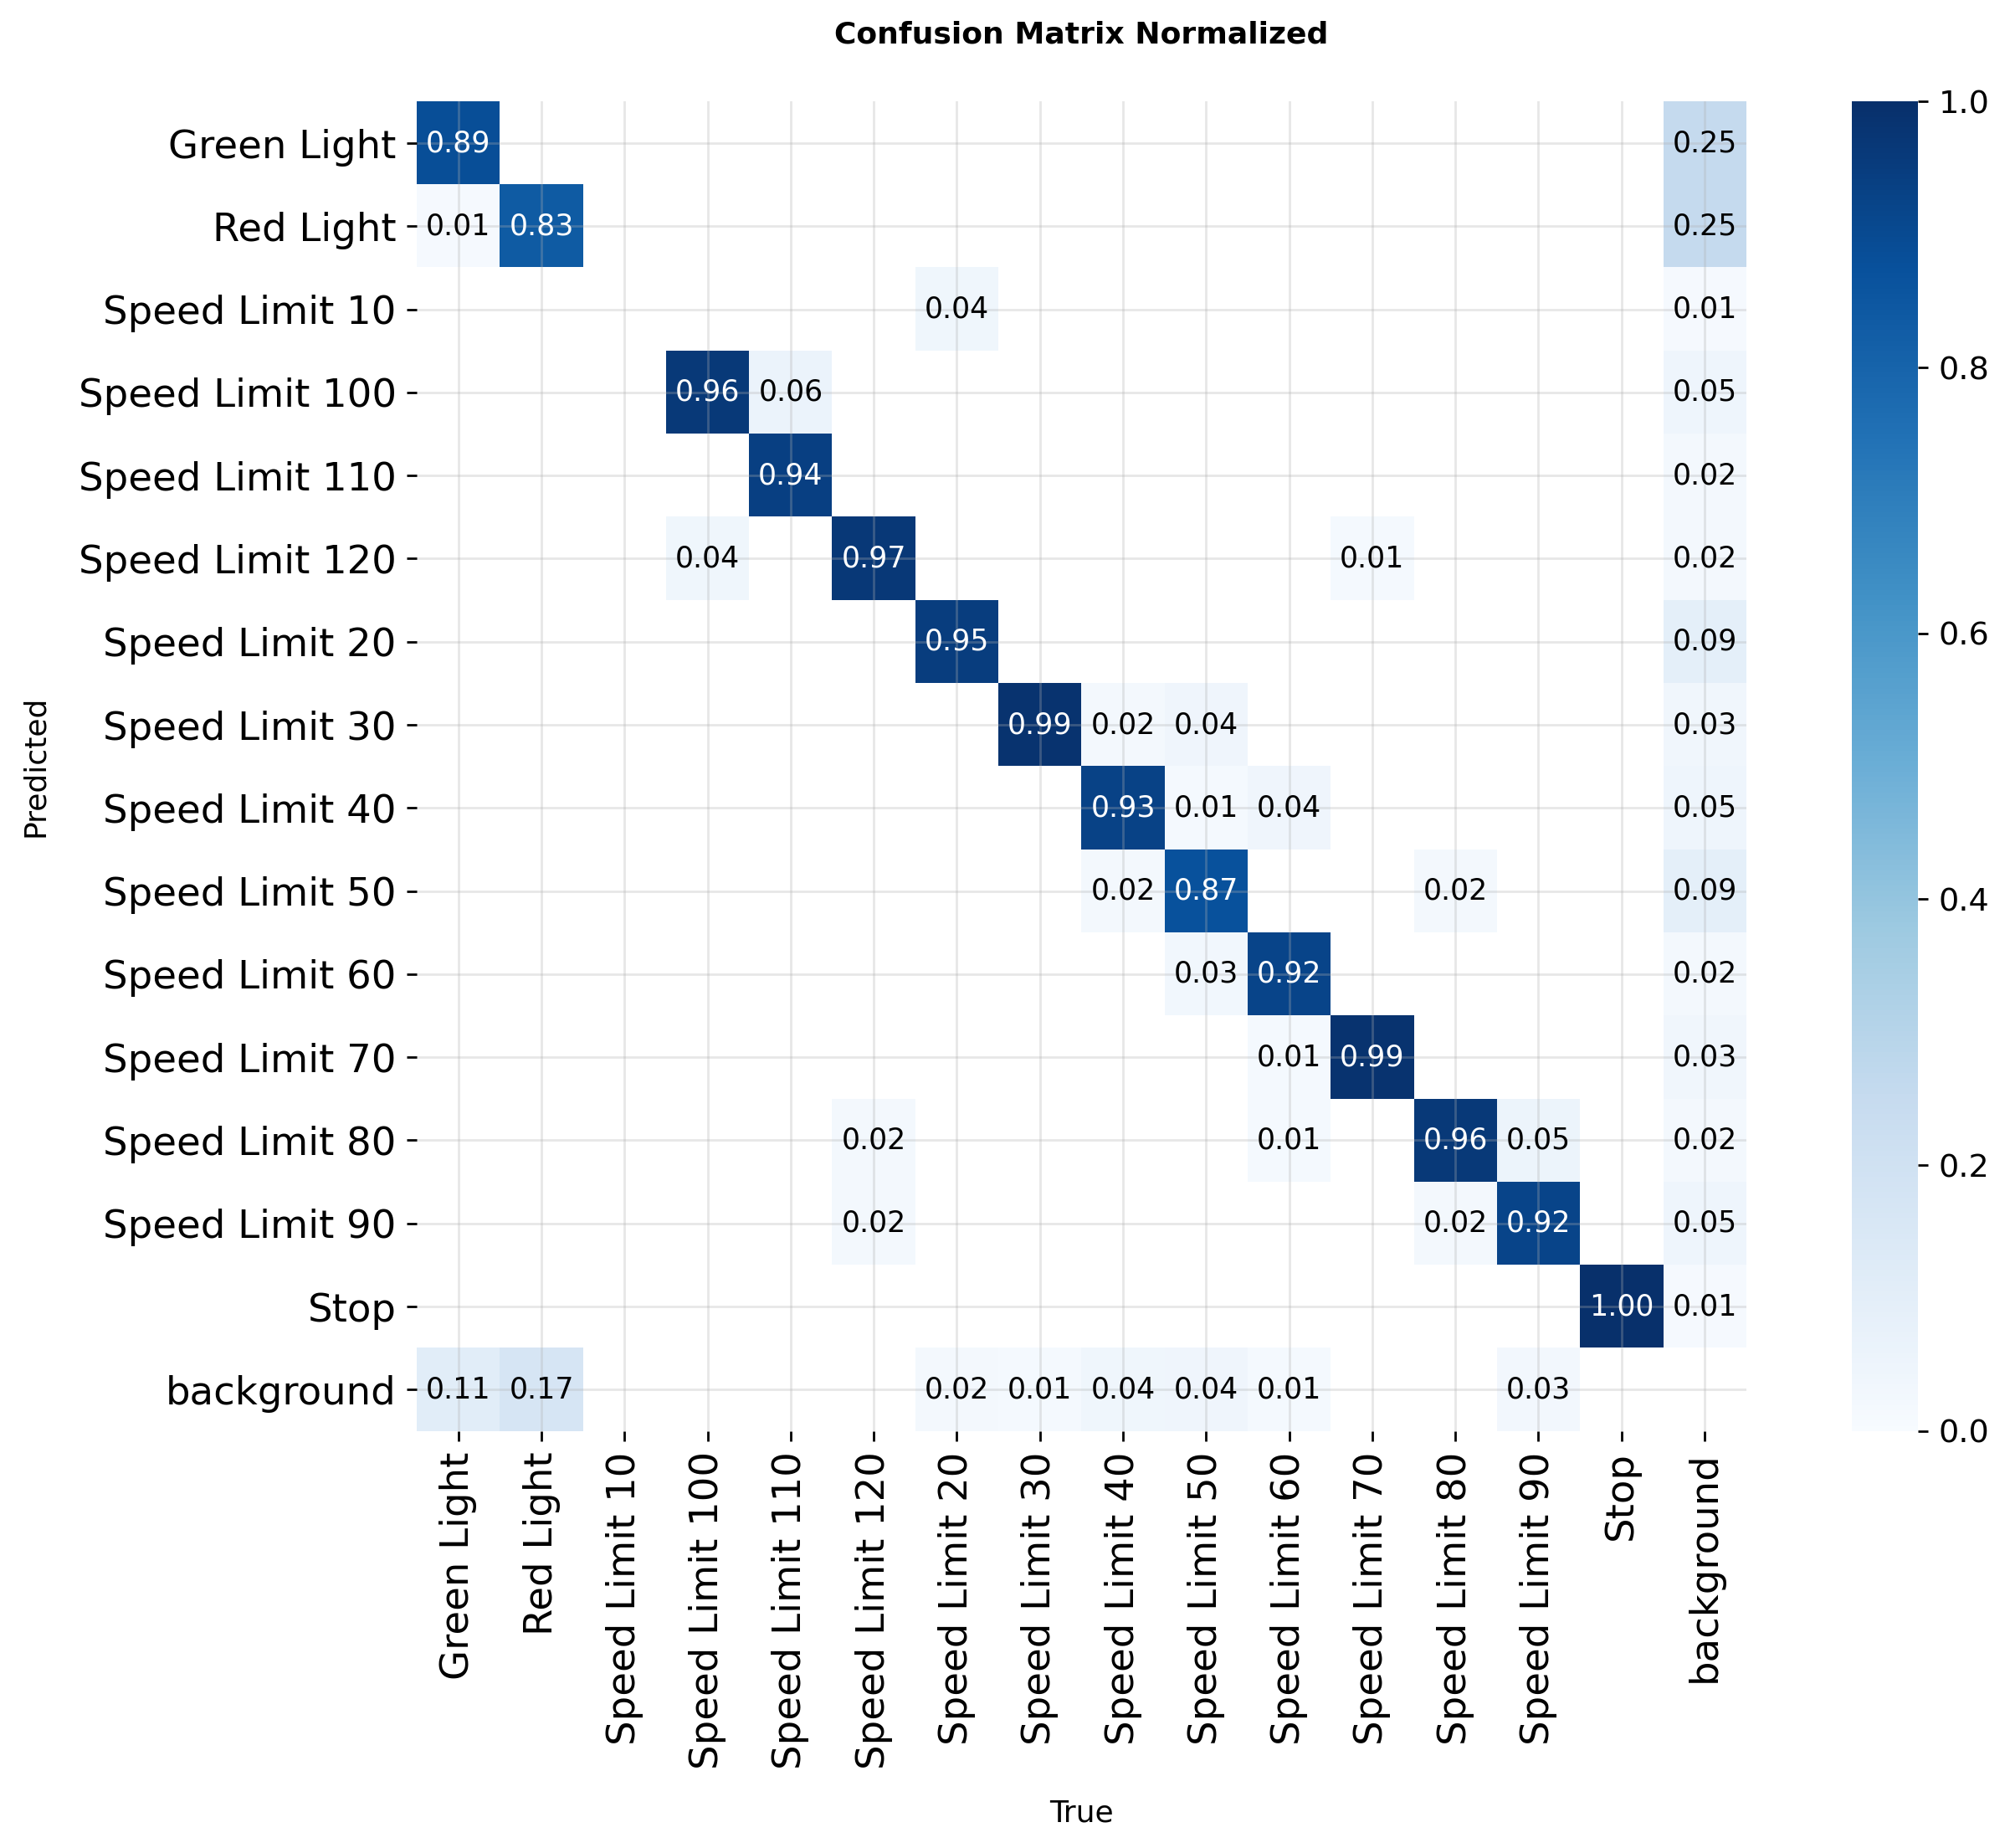
\includegraphics[width=0.88\textwidth]{figures/yolo_confusion_norm.png}
\caption{Ma trận nhầm lẫn chuẩn hoá trên tập kiểm định}
\label{fig:confusion}
\end{figure}

Ma trận nhầm lẫn ở Hình~\ref{fig:confusion} cho thấy đường chéo chính chiếm ưu thế rõ rệt. Các nhầm
lẫn còn lại tập trung vào nhóm biển giới hạn tốc độ. Điều này hợp lý về mặt thị giác: mười ba lớp
giới hạn tốc độ có hình dạng, màu sắc và viền hoàn toàn giống nhau, chỉ khác ở chữ số bên trong. Ở
độ phân giải thấp, chữ số là chi tiết đầu tiên bị mất, trong khi hình tròn viền đỏ vẫn nhận ra
được. Nói cách khác, mô hình \emph{định vị} tốt hơn \emph{phân loại}.

Quan sát này củng cố thêm cho kết luận ở Mục~\ref{sec:ap_nho_ket_qua}: khi vật thể nhỏ đi hoặc khi
biểu diễn bị nhiễu do lượng tử hoá, phần thông tin mất đầu tiên chính là chi tiết nhỏ bên trong
biển --- thứ quyết định phân loại đúng hay sai.

\subsection{Ảnh hưởng của mất cân bằng lớp}

Lớp \textit{Speed Limit 10} chỉ có 22 mẫu trên toàn bộ dữ liệu, tương đương khoảng 15 mẫu trong tập
huấn luyện. Với số lượng này, mô hình khó học được biểu diễn ổn định, và bất kỳ chỉ số nào tính
riêng cho lớp đó đều có phương sai rất lớn. Đây là biểu hiện điển hình của bài toán mất cân bằng
lớp trong học sâu~\cite{johnson2019imbalance}.

Cần lưu ý rằng mAP lấy trung bình \emph{không có trọng số} trên các lớp, nên một lớp thiểu số có
$AP$ thấp sẽ kéo mAP tổng xuống ngang bằng với một lớp đa số.

\subsection{Rò rỉ dữ liệu giữa các tập}

Thủ tục kiểm toán mô tả ở Mục~\ref{sec:kiem_toan_ro_ri} cho kết quả đáng lo ngại.

\begin{table}[H]
\centering
\caption{Kết quả kiểm toán rò rỉ dữ liệu giữa các tập}
\label{tab:ro_ri}
\small
\begin{tabular}{lr}
\toprule
\textbf{Hạng mục} & \textbf{Số lượng} \\
\midrule
Nhóm ảnh nguồn xuất hiện ở nhiều hơn một tập & 155 \\
Trong đó trùng byte hoàn toàn                & 101 \\
Ảnh kiểm tra có bản sao trong tập huấn luyện & \textbf{65 / 638 (10,2\%)} \\
Tập kiểm tra thực sự sạch còn lại            & \textbf{573 ảnh} \\
\bottomrule
\end{tabular}
\end{table}

Mô hình đã nhìn thấy đúng 65 ảnh đó trong lúc huấn luyện, nên phần dự đoán trên chúng thiên về ghi
nhớ hơn là khái quát hoá. Mọi con số mAP trong báo cáo này vì vậy nên được hiểu là \emph{cận trên}.

Điểm nhẹ nhõm duy nhất: vì rò rỉ ảnh hưởng \emph{như nhau} tới cả năm cấu hình --- chúng dùng chung
một tập kiểm tra --- nên các phép so sánh tương đối ở Bảng~\ref{tab:delta} vẫn giữ nguyên giá trị.
Cái bị ảnh hưởng là giá trị tuyệt đối, không phải thứ tự xếp hạng.

\section{Kiểm chứng trên video đường thật}
\label{sec:video}

Toàn bộ kết quả ở các mục trên được đo trên tập kiểm tra, vốn có cùng phân bố với tập huấn luyện.
Mục này kiểm chứng luận điểm trung tâm --- rằng điểm yếu thật nằm ở vật thể nhỏ --- trên dữ liệu
\emph{ngoài phân bố}: ba đoạn video đường phố thu bằng camera hành trình.

\subsection{Thiết kế phép kiểm chứng}

\begin{table}[H]
\centering
\caption{Ba video dùng để kiểm chứng}
\label{tab:video_meta}
\small
\begin{tabular}{lrrrr}
\toprule
\textbf{Tệp} & \textbf{Độ phân giải} & \textbf{Tốc độ khung} & \textbf{Số khung} & \textbf{Thời lượng} \\
\midrule
A.mp4        & 1660$\times$1244 & 24 & 121 & 5,0 s \\
B.mp4        & 1280$\times$720  & 24 & 240 & 10,0 s \\
download.mp4 & 1080$\times$1920 & 30 & 500 & 16,7 s \\
\bottomrule
\end{tabular}
\end{table}

\hopnhanmanh{Ba video này \textbf{không có nhãn thật}. Vì vậy mục này \emph{không} báo cáo mAP hay
bất kỳ độ đo chính xác nào --- làm vậy sẽ là bịa số. Thay vào đó, phép kiểm chứng được thiết kế
quanh những đại lượng quan sát được mà không cần nhãn, và quanh một dự đoán có thể sai: \emph{nếu}
điểm yếu thật nằm ở vật thể nhỏ, thì việc tăng độ phân giải đầu vào phải làm lộ ra thêm các phát
hiện có \textbf{cạnh nhỏ} một cách chọn lọc, chứ không làm tăng đều số phát hiện ở mọi cỡ.}

Ba cấu hình suy luận được so sánh, xử lý một trong mỗi mười khung hình, tổng cộng 87 khung hình cho
mỗi cấu hình:

\begin{itemize}[leftmargin=1.5cm]
\item \textbf{Cấu hình A} --- kích thước ảnh 640, ngưỡng tin cậy 0,35, không cắt vùng quan tâm.
\item \textbf{Cấu hình B} --- kích thước ảnh 1280, ngưỡng tin cậy 0,20, cắt bỏ 30\% đáy khung hình
(vùng mặt đường và nắp ca-pô, không chứa biển báo).
\item \textbf{Cấu hình C} --- như B, cộng thêm suy luận theo lát cắt: khung hình được chia thành các
ô 640 điểm ảnh chồng lấn 20\%, mỗi ô chạy qua mô hình ở tỉ lệ gốc, kèm một lượt trên toàn khung
hình, rồi gộp bằng NMS theo từng lớp.
\end{itemize}

Cần nói rõ: phép kiểm chứng này dùng trọng số của mô hình nền YOLOv8n trong ứng dụng trình diễn,
\emph{không phải} các mô hình YOLO26 ở những mục trên. Nó vì vậy không so sánh được trực tiếp với
Bảng~\ref{tab:tongquan}; mục đích của nó là kiểm chứng một \emph{cơ chế}, không phải xếp hạng mô
hình.

\subsection{Kết quả}

\begin{table}[H]
\centering
\caption{Kết quả trên 87 khung hình mỗi cấu hình, tổng hợp cả ba video}
\label{tab:video_tong}
\small
\begin{tabular}{lrrrrr}
\toprule
\textbf{Cấu hình} & \textbf{Số phát hiện} & \textbf{Trên mỗi khung} & \textbf{Tin cậy TB} & \textbf{Cạnh trung vị} & \textbf{Số lớp} \\
\midrule
A --- 640, conf 0,35   & 185 & 2,13 & 0,618 & 4,49\% & 13 \\
B --- 1280, conf 0,20  & 431 & 4,95 & 0,633 & 3,00\% & 14 \\
C --- 1280 + lát cắt   & \textbf{644} & \textbf{7,40} & 0,616 & \textbf{2,84\%} & 14 \\
\bottomrule
\end{tabular}
\end{table}

Số phát hiện tăng 2,3 lần từ A sang B và 3,5 lần từ A sang C. Nhưng con số quan trọng hơn nằm ở cột
cuối: \textbf{cạnh trung vị của vật thể được phát hiện giảm} từ 4,49\% xuống 2,84\% cạnh khung hình.
Nói cách khác, các cấu hình mới không chỉ tìm được \emph{nhiều} biển hơn mà còn tìm được biển
\emph{nhỏ hơn}.

\begin{figure}[H]
\centering
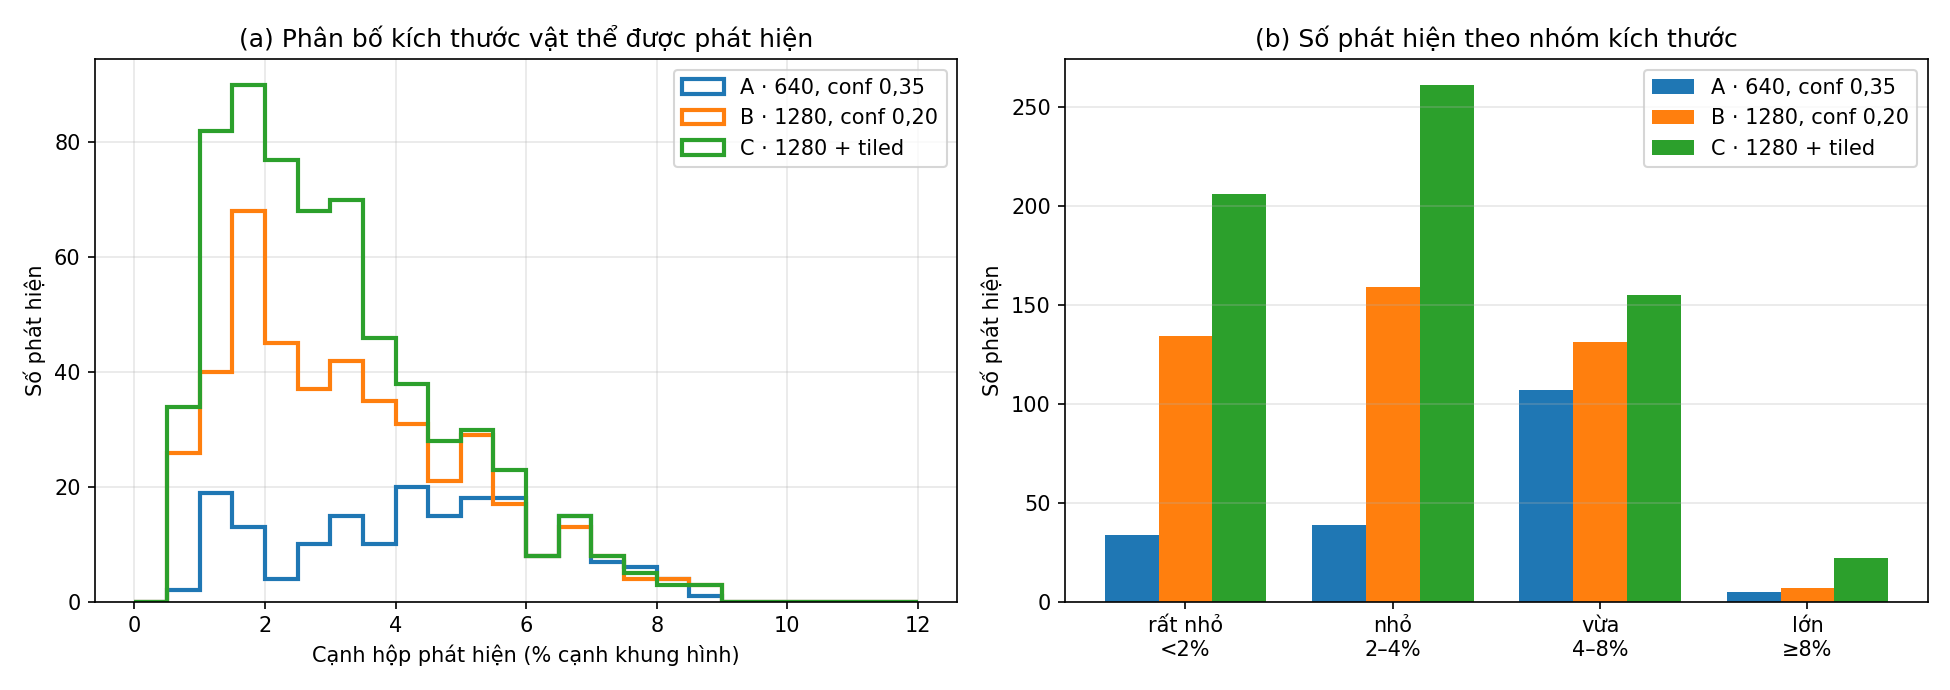
\includegraphics[width=\textwidth]{figures/video_size_dist.png}
\caption{Phân bố kích thước vật thể được phát hiện trên video đường thật}
\label{fig:video_size}
\end{figure}

\subsection{Mức tăng phân bố không đều theo kích thước}

Bảng~\ref{tab:video_bucket} là kết quả then chốt của mục này.

\begin{table}[H]
\centering
\caption{Số phát hiện theo nhóm kích thước và tỉ lệ tăng so với cấu hình A}
\label{tab:video_bucket}
\small
\begin{tabular}{lrrrr}
\toprule
\textbf{Nhóm cạnh hộp} & \textbf{A} & \textbf{B} & \textbf{C} & \textbf{Tăng A$\rightarrow$C} \\
\midrule
Rất nhỏ ($<2\%$)      & 34  & 134 & 206 & \textbf{6,1$\times$} \\
Nhỏ ($2$--$4\%$)      & 39  & 159 & 261 & \textbf{6,7$\times$} \\
Vừa ($4$--$8\%$)      & 107 & 131 & 155 & 1,4$\times$ \\
Lớn ($\ge 8\%$)       & 5   & 7   & 22  & --- \\
\bottomrule
\end{tabular}
\end{table}

\hopnhanmanh{Nhóm vật thể vừa chỉ tăng \textbf{1,4 lần}, trong khi hai nhóm nhỏ tăng \textbf{6,1 và
6,7 lần}. Mức tăng hoàn toàn không đồng đều, và nó dồn đúng vào nhóm mà lý thuyết ở
Mục~\ref{sec:vat_the_nho} đã dự đoán. Đây là kiểm chứng độc lập cho luận điểm trung tâm của báo
cáo, thu được trên dữ liệu ngoài phân bố và không cần nhãn thật.}

\subsection{Các phát hiện thêm có phải dương tính giả không?}

Đây là phản biện hiển nhiên và cần được trả lời nghiêm túc: vì cấu hình B và C hạ ngưỡng tin cậy từ
0,35 xuống 0,20, một phần các phát hiện thêm có thể chỉ là nhiễu. Không có nhãn thật thì không thể
loại trừ khả năng này hoàn toàn. Tuy nhiên có hai lập luận đáng cân nhắc.

\textbf{Thứ nhất, độ tin cậy trung bình không sụt.} Nếu các phát hiện thêm chủ yếu là nhiễu ở gần
ngưỡng, trung bình phải kéo về phía 0,20. Thực tế nó giữ nguyên và thậm chí nhích lên: 0,618 ở cấu
hình A so với 0,633 ở cấu hình B, dù sàn ngưỡng đã thấp hơn 15 điểm phần trăm. Điều này hàm ý phần
lớn phát hiện mới có điểm cao, tức mô hình \emph{thực sự} nhìn thấy chúng chứ không đoán mò.

\textbf{Thứ hai, tính chọn lọc theo kích thước là chữ ký của tín hiệu thật.} Nhiễu do hạ ngưỡng sẽ
phân bố tương đối đều theo kích thước. Ở đây nhóm vừa gần như đứng yên trong khi nhóm nhỏ tăng gấp
sáu lần --- đúng dạng phân bố mà cơ chế ``vật thể nhỏ mất chi tiết khi ảnh bị co'' dự đoán, và không
phải dạng mà nhiễu ngẫu nhiên tạo ra.

Dù vậy, kết luận đúng mực vẫn là: \emph{dữ liệu quan sát được nhất quán với giả thuyết vật thể nhỏ},
chứ chưa phải bằng chứng dứt điểm. Muốn khẳng định chắc chắn phải gán nhãn thủ công một tập khung
hình và tính $AP$ thật --- việc này được đưa vào hướng phát triển ở Chương~\ref{ch:tong_ket}.

\subsection{Quan sát định tính}

\begin{figure}[H]
\centering
\begin{subfigure}[b]{0.48\textwidth}
  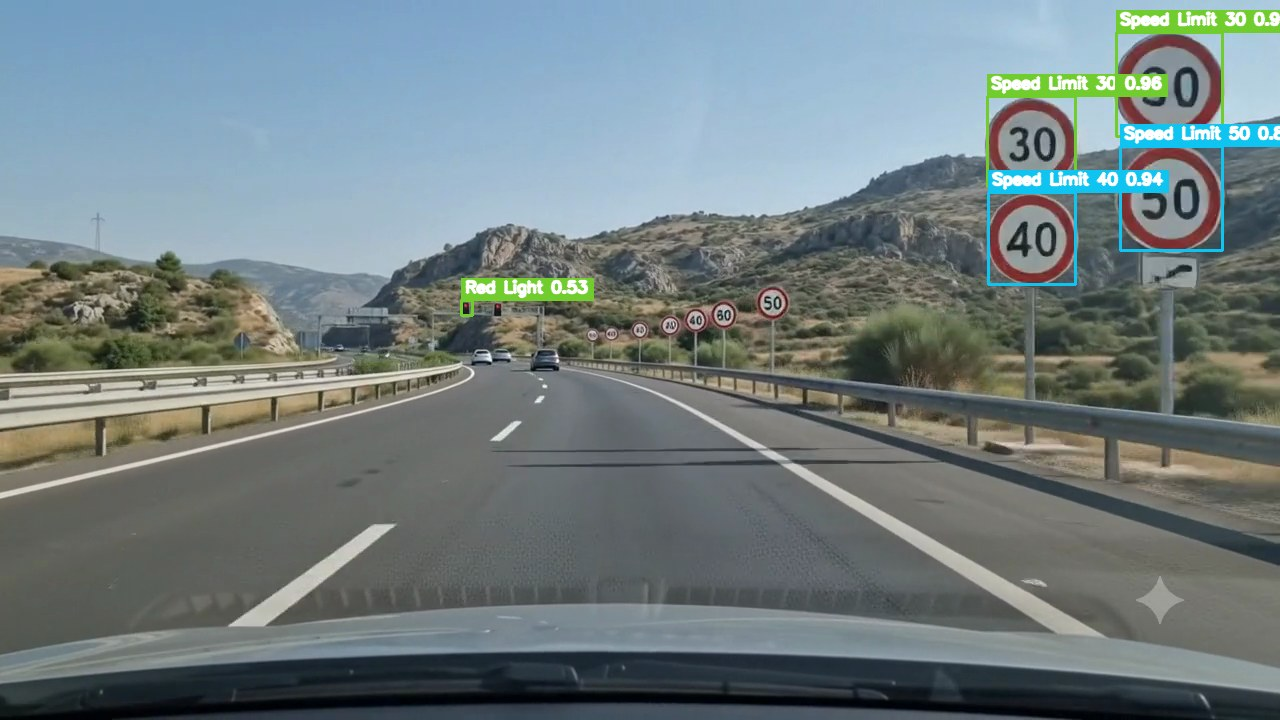
\includegraphics[width=\textwidth]{figures/video_frame_640.jpg}
  \caption{Cấu hình A --- 5 phát hiện}
\end{subfigure}
\hfill
\begin{subfigure}[b]{0.48\textwidth}
  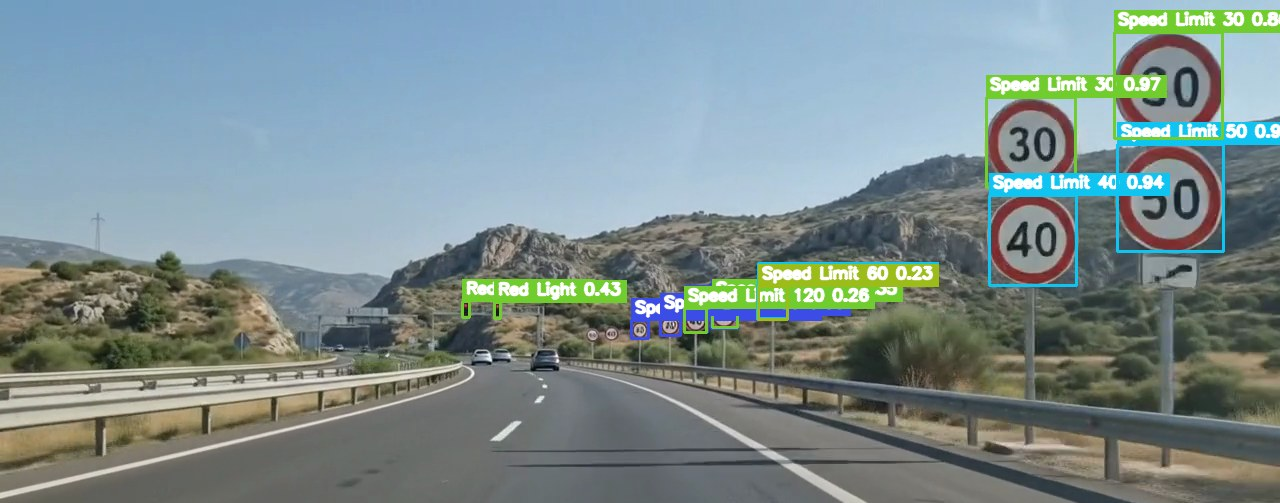
\includegraphics[width=\textwidth]{figures/video_frame_1280.jpg}
  \caption{Cấu hình B --- 16 phát hiện}
\end{subfigure}
\caption{Cùng một khung hình của \texttt{B.mp4} qua hai cấu hình suy luận}
\label{fig:video_frame}
\end{figure}

Hình~\ref{fig:video_frame} minh hoạ rõ hiện tượng. Cụm biển ở gần bên phải khung hình được phát hiện
với độ tin cậy rất cao (0,94 đến 0,97) ở cả hai cấu hình --- đây là chế độ ``biển lớn'' mà mô hình đã
được dạy rất kỹ, đúng như phân tích thành phần dữ liệu ở Mục~\ref{sec:thanhphan} đã chỉ ra. Ngược
lại, cụm biển ở xa giữa khung hình chỉ xuất hiện ở cấu hình B và với độ tin cậy thấp hơn hẳn (0,23
đến 0,43). Khoảng cách về độ tin cậy giữa hai nhóm --- hơn gấp đôi --- cho thấy mô hình ``chắc chắn''
với biển gần và ``lưỡng lự'' với biển xa, dù cả hai đều là biển thật.

Một quan sát nữa đáng ghi nhận: 14 trong số 15 lớp xuất hiện trong kết quả, và lớp được phát hiện
nhiều nhất là \textit{Red Light} với 110 lần ở cấu hình B. Tuy nhiên đây cũng là lớp có nhiều khả
năng bị dương tính giả nhất trên cảnh đường cao tốc, nơi hầu như không có đèn tín hiệu --- một dấu
hiệu nữa cho thấy cần nhãn thật trước khi kết luận về độ chính xác.

\section{Bàn luận}

Đối chiếu với các công trình đã nêu ở Chương~\ref{ch:co_so}, kết quả của đề tài tương đồng ở hai
điểm và bổ sung thêm một điểm.

Điểm tương đồng thứ nhất là về điều kiện áp dụng của chưng cất tri thức. Bài báo
gốc~\cite{hinton2015distillation} xây dựng lập luận trên giả định tồn tại một mô hình thầy đủ mạnh
và một khoảng cách năng lực đáng kể. Thực nghiệm ở đây, với khoảng cách chỉ 1,72 điểm phần trăm,
rơi ra ngoài vùng giả định đó và cho kết quả âm --- không mâu thuẫn với lý thuyết mà minh hoạ cho
giới hạn của nó.

Điểm tương đồng thứ hai là về lượng tử hoá. Các nghiên cứu về lượng tử hoá số
nguyên~\cite{jacob2018quantization} nêu rõ rằng lợi ích tốc độ phụ thuộc vào nhân tính toán của
phần cứng đích, nhưng điều này thường bị lược bỏ trong các trình bày phổ thông. Thí nghiệm ở đây
ghi nhận INT8 \emph{chậm hơn} FP32 hơn hai lần, đúng như cảnh báo đó.

Điểm bổ sung, và cũng là đóng góp riêng của đề tài, nằm ở cách đo. Các báo cáo về nén mô hình
thường tổng kết bằng một câu dạng ``giảm 70\% dung lượng, chỉ mất 0,4\% mAP''. Kết quả ở đây cho
thấy câu tổng kết đó, dù không sai, vẫn có thể gây hiểu nhầm nghiêm trọng: cùng phép can thiệp ấy
làm $AP$ trên vật thể nhỏ giảm gấp 6,5 lần. Với những bài toán mà vật thể nhỏ mới là trường hợp
quan trọng --- phát hiện biển báo giao thông là một ví dụ điển hình --- việc chỉ báo cáo mAP tổng là
không đủ. Kiến nghị rút ra là mọi báo cáo về nén mô hình cho bài toán phát hiện nên kèm $AP$ tách
theo nhóm kích thước, và chi phí bổ sung để có chỉ số này gần như bằng không nếu đã dùng bộ đánh
giá COCO.
